\documentclass[aspectratio=169,10pt]{beamer}
\usetheme{metropolis}
\metroset{numbering=fraction, progressbar=foot, block=fill, sectionpage=none, subsectionpage=none}

\usepackage{booktabs}
\usepackage{amsmath,amssymb}
\usepackage{tikz}
\usetikzlibrary{positioning,arrows.meta,calc,fit,backgrounds}
\usepackage{graphicx}
\usepackage{pgfpages}
\graphicspath{{figs/}}

% Compact, readable monospaced inline
\usepackage[scaled=0.85]{beramono}

% --- Speaker notes ---------------------------------------------------------
% Default: slides only. Uncomment one of the lines below to render notes:
%   \setbeameroption{show notes}                        % notes interleaved
%   \setbeameroption{show only notes}                   % notes-only PDF
%   \setbeameroption{show notes on second screen=right} % slide + notes side-by-side
% ---------------------------------------------------------------------------

% Section colors
\definecolor{accent}{HTML}{A84425}
\definecolor{good}{HTML}{2F7A46}
\definecolor{bad}{HTML}{A83232}
\definecolor{muted}{HTML}{645A54}
\setbeamercolor{progress bar}{fg=accent}
\setbeamercolor{title separator}{fg=accent}
\setbeamercolor{frametitle}{bg=black!90,fg=white}

\title{Distillation and Edge-Aware Loss\\for Efficient Monocular Depth Estimation}
\subtitle{ECE 4990 -- Cal Poly Pomona, Spring 2026}
\author{Alexander Assal \and Parsa Ghasemi}
\institute{Department of Electrical and Computer Engineering\\
\texttt{arassal@cpp.edu} \quad \texttt{mghasemi@cpp.edu}\\[0.5em]
\textcolor{accent}{\texttt{github.com/arassal/depth-project}}}
\date{}

\begin{document}

\maketitle
\note{%
[AA] Good afternoon. I'm Alexander Assal, and this is Parsa Ghasemi. Our project for
ECE 4990 is \emph{Distillation and Edge-Aware Loss for Efficient Monocular Depth
Estimation}. The full source, paper, and slides are on GitHub at
\texttt{arassal/depth-project}. We'll walk you through the problem, our method,
the experiments, and what we learned.
}

% --------------------------------------------------------------------------
\begin{frame}{Outline}
\begin{itemize}
  \item Problem: monocular relative depth from a single RGB image
  \item Method: distill Depth Anything Large $\rightarrow$ Small with multi-scale gradient supervision
  \item Datasets: NYU-v2 (indoor) and KITTI eigen subset (outdoor)
  \item Three-axis hyperparameter sweep over $\alpha$, $\beta$, learning rate
  \item Main finding: \textbf{learning rate dominates loss balance in small-data distillation}
\end{itemize}
\end{frame}
\note{%
[PG] Here's the path we'll take. First the problem -- why single-image depth
estimation is hard. Then our method: we distill a large pretrained model into a
small one with an extra gradient supervision term. Then datasets -- NYU-v2
indoors and KITTI outdoors. Then our three-axis sweep over the distillation
weight $\alpha$, the gradient weight $\beta$, and the learning rate. The main
finding in one sentence: in the small-data regime, the learning rate dominates
the loss balance. I'll come back to that at the end.
}

% --------------------------------------------------------------------------
\section{Problem}

\begin{frame}{Monocular depth is ill-posed}
\begin{itemize}
  \item A single RGB image is consistent with infinitely many world geometries
  \item Recovery is up to scale $+$ shift unless additional information is given
  \item Modern systems train relative depth and align scale at evaluation
\end{itemize}
\vspace{0.4em}
\begin{block}{Foundation model used here}
\textbf{Depth Anything} (Yang et al., CVPR 2024) -- DPT head on DINOv2 ViT backbone,
trained on 1.5M labeled + 62M pseudo-labeled images.
\begin{itemize}
  \item \textbf{Small} -- $\sim$25M params -- our \emph{student}, deployable on 4\,GB GPU
  \item \textbf{Large} -- $\sim$335M params -- our \emph{teacher}, frozen
\end{itemize}
\end{block}
\end{frame}
\note{%
[PG] Monocular depth estimation predicts a per-pixel depth map from a single
RGB image. The catch is that a single image is consistent with infinitely many
world geometries -- without stereo, intrinsics, or active sensing, you can only
recover depth up to an unknown scale and shift. Modern systems sidestep this by
training for \emph{relative} depth and aligning the scale at evaluation time.

The foundation model we build on is Depth Anything -- Yang et al., CVPR 2024.
It's a DPT depth head on a self-supervised DINOv2 backbone, trained on 1.5
million labeled images plus 62 million pseudo-labeled images. We use the Small
variant, about 25 million parameters, as our \textbf{student} -- it fits on a
4-gigabyte laptop GPU -- and the Large variant, about 335 million parameters,
as our frozen \textbf{teacher}.
}

% --------------------------------------------------------------------------
\section{Related Work}

\begin{frame}{Related work}
\begin{columns}[T,onlytextwidth]
\begin{column}{0.48\textwidth}
\textbf{Backbone lineage}
\begin{itemize}\setlength{\itemsep}{0.25em}
  \item Eigen et al.\ 2014 -- first deep monocular depth
  \item DPT (Ranftl 2021) -- dense prediction head
  \item DINOv2 (Oquab 2023) -- self-sup.\ ViT
  \item MiDaS (Ranftl 2022) -- relative depth + scale align
  \item Depth Anything v1/v2 (Yang 2024)
\end{itemize}
\end{column}
\begin{column}{0.48\textwidth}
\textbf{Methods we adapt}
\begin{itemize}\setlength{\itemsep}{0.25em}
  \item Hinton 2015 -- knowledge distillation
  \item Distill-Any-Depth (He 2025) -- affine-invariant output distillation
  \item ZoeDepth (Bhat 2023) -- multi-scale gradient $L_1$
  \item BTS (Lee 2019) -- silog loss
\end{itemize}
\end{column}
\end{columns}
\vspace{0.5em}
\begin{alertblock}{Our contribution}
Empirical, not architectural: a controlled three-axis study of how
distillation and gradient supervision behave in a \emph{small-data} fine-tune regime.
\end{alertblock}
\end{frame}
\note{%
[PG] Our backbone lineage starts with Eigen 2014, the first deep monocular depth
network. DPT (Ranftl 2021) introduced the dense-prediction Transformer head we
use. DINOv2 (Oquab 2023) is the self-supervised encoder. MiDaS (Ranftl 2022)
introduced the relative-depth-plus-scale-alignment evaluation we follow. Depth
Anything v1 and v2 are the pretrained checkpoints.

On the method side we adapt two pieces from the literature. Affine-invariant
output distillation comes from Distill-Any-Depth, He et al.\ 2025. The
multi-scale gradient $L_1$ loss comes from ZoeDepth, Bhat et al.\ 2023. Our
contribution is \emph{not} a new architecture -- it's an empirical study of how
these two pieces behave when you fine-tune on a small dataset.
}

% --------------------------------------------------------------------------
\section{Method}

\begin{frame}{Architecture: teacher--student distillation}
\centering
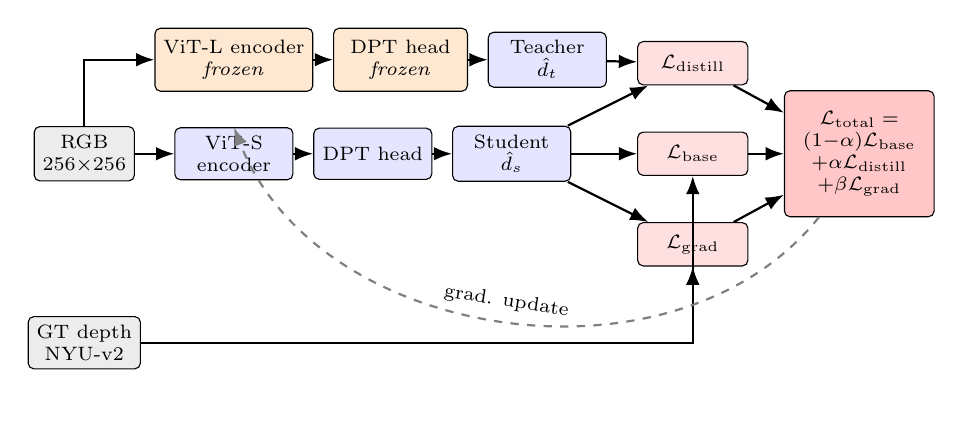
\begin{tikzpicture}[
  font=\scriptsize,
  >=Latex,
  block/.style={draw, rounded corners=2pt, align=center, inner sep=3pt,
                fill=blue!10, minimum height=0.65cm, minimum width=1.5cm},
  bigblock/.style={draw, rounded corners=2pt, align=center, inner sep=3pt,
                   fill=orange!18, minimum height=0.8cm, minimum width=1.7cm},
  loss/.style={draw, rounded corners=2pt, align=center, inner sep=3pt,
               fill=red!12, minimum height=0.55cm, minimum width=1.4cm},
  io/.style={draw, rounded corners=2pt, align=center, inner sep=3pt,
             fill=gray!15, minimum height=0.6cm, minimum width=1.2cm},
  arrow/.style={->, thick},
]
% Inputs
\node[io] (rgb) at (0,0) {RGB\\ $256{\times}256$};
\node[io] (gt)  at (0,-2.4) {GT depth\\ NYU-v2};

% Student
\node[block, right=0.5cm of rgb] (s_enc) {ViT-S\\ encoder};
\node[block, right=0.25cm of s_enc] (s_dec) {DPT head};
\node[block, right=0.25cm of s_dec] (s_out) {Student\\ $\hat d_s$};

% Teacher
\node[bigblock, above=0.45cm of s_enc] (t_enc) {ViT-L encoder\\ \emph{frozen}};
\node[bigblock, right=0.25cm of t_enc] (t_dec) {DPT head\\ \emph{frozen}};
\node[block, right=0.25cm of t_dec] (t_out) {Teacher\\ $\hat d_t$};

% Losses
\node[loss] (l_dist) at ($(s_out)+(2.3,1.15)$) {$\mathcal{L}_{\text{distill}}$};
\node[loss] (l_base) at ($(s_out)+(2.3,0)$) {$\mathcal{L}_{\text{base}}$};
\node[loss] (l_grad) at ($(s_out)+(2.3,-1.15)$) {$\mathcal{L}_{\text{grad}}$};

\node[draw, rounded corners=2pt, fill=red!22, right=0.45cm of l_base,
      minimum height=1.6cm, minimum width=1.9cm, align=center] (total)
      {$\mathcal{L}_{\text{total}}=$\\$(1{-}\alpha)\mathcal{L}_{\text{base}}$\\$+\alpha\mathcal{L}_{\text{distill}}$\\$+\beta\mathcal{L}_{\text{grad}}$};

% Flows
\draw[arrow] (rgb) -- (s_enc);
\draw[arrow] (s_enc) -- (s_dec);
\draw[arrow] (s_dec) -- (s_out);
\draw[arrow] (rgb.north) |- (t_enc.west);
\draw[arrow] (t_enc) -- (t_dec);
\draw[arrow] (t_dec) -- (t_out);

\draw[arrow] (s_out) -- (l_dist);
\draw[arrow] (t_out) -- (l_dist);
\draw[arrow] (s_out) -- (l_base);
\draw[arrow] (gt) -| (l_base);
\draw[arrow] (s_out) -- (l_grad);
\draw[arrow] (gt) -| (l_grad);

\draw[arrow] (l_dist) -- (total);
\draw[arrow] (l_base) -- (total);
\draw[arrow] (l_grad) -- (total);

\draw[->, dashed, thick, draw=gray] (total) to[bend left=60] node[above, sloped] {\scriptsize grad. update} (s_enc.north);
\end{tikzpicture}

\vspace{0.4em}
\footnotesize Same RGB feeds both networks. Teacher is loaded once and held in
\texttt{eval()} with \texttt{requires\_grad=False}. Student is the only model with trainable weights.
\end{frame}
\note{%
[AA] Here's our pipeline. The same RGB image feeds two networks in parallel.
On the bottom is the \textbf{student} -- Depth Anything Small, in blue -- the
only model with trainable weights. On top is the \textbf{teacher} -- Depth
Anything Large, in orange -- loaded once and frozen.

Both produce a depth prediction. We compute three losses. $\mathcal{L}_{\text{base}}$ compares the
student to NYU-v2 ground truth. $\mathcal{L}_{\text{distill}}$ compares the student to the teacher's
prediction. $\mathcal{L}_{\text{grad}}$ is a multi-scale gradient loss against GT. They're
combined with weights $\alpha$ and $\beta$. Only the student's gradient flows back
through the encoder. The teacher exists purely as a dense, low-noise per-pixel
supervision signal -- it never sees gradient updates.
}

% --------------------------------------------------------------------------
\begin{frame}{Loss function}
\begin{block}{Total loss}
\[
\mathcal{L}_{\text{total}} \;=\; (1-\alpha)\,\mathcal{L}_{\text{base}}(\hat d_s, d_{\text{gt}})
\;+\; \alpha\,\mathcal{L}_{\text{distill}}(\hat d_s, \hat d_t)
\;+\; \beta\,\mathcal{L}_{\text{grad}}(\hat d_s, d_{\text{gt}})
\]
\end{block}

\textbf{Affine-invariant $L_1$} (used by $\mathcal{L}_{\text{base}}$ and $\mathcal{L}_{\text{distill}}$):
robust per-sample normalization by median + MAD, then per-pixel $L_1$.
\[
\tilde d(p) = \frac{d(p) - \operatorname{med}(d|_{\mathcal V})}{\overline{|d|_{\mathcal V} - \operatorname{med}(d|_{\mathcal V})|}}
\qquad
\mathcal{L}_{\text{ail1}} = \tfrac{1}{|\mathcal V|}\!\sum_{p\in\mathcal V}\!\big|\tilde d(p) - \tilde d^{\star}(p)\big|
\]

\textbf{Multi-scale gradient $L_1$}: penalize gradient disagreement at scales $\{1,2,4\}$.

\vspace{0.3em}
\begin{itemize}\setlength{\itemsep}{0.15em}
  \item $\alpha=0$ -- pure supervised fine-tune  \hfill $\alpha=1$ -- pure distillation
  \item $\beta$ -- second-order edge sharpening
\end{itemize}
\end{frame}
\note{%
[AA] The total loss has three terms with two mixing weights -- $(1-\alpha)$ times the
base loss, plus $\alpha$ times the distillation loss, plus $\beta$ times the gradient
loss.

Both the base and distillation losses use the same \textbf{affine-invariant} $L_1$.
We normalize each sample by its median and mean absolute deviation, \emph{then}
take the $L_1$. We're training relative depth, so two predictions that agree on
structure but disagree on overall scale should have zero loss. Median+MAD is
robust to specular pixels that would explode a mean+std version.

The gradient loss penalizes disagreement at three downsampling scales -- 1, 2,
and 4. So $\alpha=0$ is pure supervised fine-tune; $\alpha=1$ is pure distillation;
$\beta$ controls boundary sharpness.
}

% --------------------------------------------------------------------------
\begin{frame}{Training procedure}
\begin{columns}[T,onlytextwidth]
\begin{column}{0.52\textwidth}
\textbf{Optimization}
\begin{itemize}\setlength{\itemsep}{0.2em}
  \item AdamW, weight decay $10^{-4}$
  \item Gradient clip @ $L_2$ norm 1.0
  \item Batch size 1, image 256$\times$256 (fits 4\,GB GPU)
  \item 2 epochs on the PoC subset
  \item AMP mixed precision on CUDA
\end{itemize}
\end{column}
\begin{column}{0.44\textwidth}
\textbf{Sweep harness} \texttt{src/sweep.py}
\begin{itemize}\setlength{\itemsep}{0.2em}
  \item YAML grid $\rightarrow$ Cartesian product
  \item Per-run isolated artifacts
  \item \texttt{train.py} $+$ \texttt{eval.py} subprocess per point
  \item Aggregated to \texttt{results.json}
\end{itemize}
\end{column}
\end{columns}
\vspace{0.5em}
\begin{exampleblock}{Reproducibility}
\texttt{python src/train.py --config configs/distill.yaml}\\
\texttt{python src/sweep.py --base configs/distill.yaml --grid configs/sweeps/lr\_at\_alpha07.yaml --out outputs/sweeps/lr}
\end{exampleblock}
\end{frame}
\note{%
[AA] Optimization is standard: AdamW with weight decay 1e-4, gradient clipping
at $L_2$ norm 1.0, mixed precision when CUDA is available. Batch size is 1
because we run on a 4-gigabyte laptop GPU at $256{\times}256$.

On the right is the harness we wrote for the sweep. You give it a YAML grid,
it takes the Cartesian product, and runs \texttt{train.py} and \texttt{eval.py}
as subprocesses per grid point. Each run writes into its own isolated artifact
folder -- that matters; sharing output paths leads to silent corruption.
Everything aggregates into a single \texttt{results.json}.
}

% --------------------------------------------------------------------------
\section{Experiments}

\begin{frame}{Datasets and metrics}
\begin{columns}[T,onlytextwidth]
\begin{column}{0.5\textwidth}
\textbf{Datasets}
\vspace{0.3em}
\begin{table}[H]\centering\small
\begin{tabular}{lrr}
\toprule
Split & NYU-v2 & KITTI \\
\midrule
Train & 450 & --- \\
Val   & 60  & --- \\
Test  & 59  & 100 \\
\midrule
Range (m) & [0.001, 10] & [0.001, 80] \\
\bottomrule
\end{tabular}
\end{table}
Both evaluated at $256{\times}256$ for internal comparability.
\end{column}
\begin{column}{0.5\textwidth}
\textbf{Metrics} (all after per-image scale\,+\,shift align)
\begin{itemize}\setlength{\itemsep}{0.15em}
  \item $\text{AbsRel} = \tfrac{1}{N}\sum |\hat d - d|/d$\quad$\downarrow$
  \item $\text{RMSE} = \sqrt{\tfrac{1}{N}\sum (\hat d - d)^2}$\quad$\downarrow$
  \item $\delta_n = $ fraction with $\max(\hat d/d, d/\hat d) < 1.25^n$\quad$\uparrow$
\end{itemize}
\end{column}
\end{columns}
\end{frame}
\note{%
[PG] We evaluate on two datasets. NYU-v2 -- indoor scenes -- split into 450
train, 60 validation, 59 test images, depth range 0 to 10 meters. And KITTI
eigen-test -- outdoor driving -- 100 images, depth range 0 to 80 meters. Both
are evaluated at $256{\times}256$ for internal comparability.

The metrics are the standard ones, computed after per-image least-squares scale
and shift alignment. AbsRel -- mean absolute relative error -- lower is better.
RMSE -- lower is better. And the $\delta$-thresholds -- fraction of pixels
within a factor of $1.25$, $1.25^2$, or $1.25^3$ of ground truth -- higher is
better.
}

% --------------------------------------------------------------------------
\section{Results}

\begin{frame}{NYU-v2 test results (59 images, 256$\times$256)}
\begin{table}[H]\centering
\small
\begin{tabular}{lcccccc}
\toprule
Setting & $\alpha$ & $\beta$ & lr & AbsRel $\downarrow$ & $\delta_1$ $\uparrow$ & RMSE $\downarrow$ \\
\midrule
Zero-shot DA-S                          & --- & --- & ---       & 0.1550 & 0.8146 & 0.5375 \\
Distilled, default \texttt{distill.yaml} & 0.5 & 0.1 & $10^{-5}$ & \textcolor{bad}{0.2791} & \textcolor{bad}{0.6292} & \textcolor{bad}{0.8898} \\
\textbf{Distilled, best (ours)}          & 0.7 & 0.3 & $10^{-7}$ & \textcolor{good}{\textbf{0.1505}} & \textcolor{good}{\textbf{0.8164}} & \textcolor{good}{\textbf{0.5262}} \\
\bottomrule
\end{tabular}
\end{table}
\vspace{0.2em}
\begin{itemize}\setlength{\itemsep}{0.15em}
  \item Default config \emph{collapses} the student -- AbsRel almost doubles.
  \item Best swept config \emph{improves} every metric over zero-shot.
\end{itemize}
\end{frame}
\note{%
[AA] Three rows tell our headline story. Top row: zero-shot Depth Anything
Small -- AbsRel 0.155, $\delta_1$ 0.815, RMSE 0.54. That's our reference.

Middle row, in red: the \textbf{default} distillation configuration shipped in
our repo -- $\alpha=0.5$, $\beta=0.1$, lr $=10^{-5}$. AbsRel almost doubles to
0.28. $\delta_1$ drops to 0.63. RMSE jumps by 66\%. The student collapsed.

Bottom row, in green: the \textbf{best configuration we found} after the sweep.
$\alpha=0.7$, $\beta=0.3$, but the key change is the learning rate -- $10^{-7}$,
two orders of magnitude lower. AbsRel drops to 0.1505, slightly \emph{better}
than zero-shot. Every single metric moves in the right direction. The mean
improvement is small but consistent.
}

\begin{frame}{All five metrics, side by side}
\centering

\includegraphics[width=0.95\textwidth]{training/multimetric_bars.png}\\[0.3em]
\footnotesize The collapse mode hurts everything; the best-found configuration
matches or beats zero-shot on every metric.
\end{frame}
\note{%
[AA] The grouped bar chart drives the same point home visually. For every
metric -- AbsRel, RMSE, and all three $\delta$ thresholds -- the red bar
(default config) is worse than zero-shot. The green bar (our best config)
matches or beats zero-shot on every one. That's the kind of evidence that
tells you the improvement isn't an artifact of one metric -- it shows up
everywhere we look.
}

% --------------------------------------------------------------------------
\begin{frame}{Training collapse at default learning rate}
\centering

\includegraphics[width=0.95\textwidth]{training/training_curves_default.png}\\[0.3em]
\begin{itemize}\setlength{\itemsep}{0.15em}
  \item Epoch 1 tracks zero-shot ($\approx 0.157$ val AbsRel).
  \item Epoch 2: val AbsRel $\to 1.0$, $\delta_1 \to 0$ -- student saturates to near-constant.
  \item Trigger: batch $=1$ $+$ 450-image train set $+$ lr $=10^{-5}$.
\end{itemize}
\end{frame}
\note{%
[AA] Why does the default config fail so badly? Look at the training curves.

Left panel: training loss decreasing normally over two epochs -- looks fine.
Middle panel: validation AbsRel. At epoch 1 it tracks zero-shot at 0.157. At
epoch 2 it shoots up to 1.0. Right panel: validation $\delta_1$. At epoch 1
about 0.82. At epoch 2 it drops to literally zero.

That signature -- val AbsRel saturating at 1.0 and $\delta_1$ at 0 -- is the
student emitting a near-constant prediction. The trigger is the combination of
batch size 1, 450 training images, and learning rate $10^{-5}$. A few
high-curvature mini-batches late in epoch 2 push the encoder into a degenerate
region.
}

\begin{frame}{Loss component decomposition}
\centering

\includegraphics[width=0.78\textwidth]{training/loss_components.png}\\[0.3em]
\footnotesize Base and distill losses contribute comparably ($\approx 1.0$ per batch at
epoch 2); the multi-scale gradient term is a smaller boundary signal ($\sim 0.5$).
\end{frame}
\note{%
[AA] Here's how the three loss terms contribute. At epoch 1 the total
per-batch loss is around 3.37 -- base about 1.36, distillation about 1.35,
gradient about 0.66. At epoch 2 they all decrease together to about 2.59. The
takeaway: base and distillation are comparable in magnitude -- they're telling
the student roughly the same story. The gradient term is smaller, as it should
be -- it's boundary sharpening, not the main objective.
}

\begin{frame}{What the default collapse looks like, per image}
\centering

\includegraphics[width=0.50\textwidth]{training/absrel_histogram_comparison.png}\hfill

\includegraphics[width=0.46\textwidth]{training/per_image_scatter_default.png}\\[0.3em]
\footnotesize \textbf{Left}: histogram shifts right $+$ grows a heavy tail.\quad
\textbf{Right}: 58 of 59 test images get worse (above $y=x$). The collapse is uniform,
not driven by outliers.
\end{frame}
\note{%
[AA] To make the collapse concrete: on the left, a histogram of per-image
AbsRel -- zero-shot in blue, default distill in orange. Blue is tight around
0.155. Orange shifts right \emph{and} grows a heavy tail past 0.4.

On the right, the same data as a scatter -- zero-shot AbsRel on $x$, distilled
on $y$, dotted $y=x$ line. \textbf{Fifty-eight of fifty-nine test images get
worse.} Only one is better. This isn't outlier-driven. The collapse is uniform
across the test set.
}

% --------------------------------------------------------------------------
\begin{frame}{Ablation: distillation weight $\alpha$}
\begin{columns}[T,onlytextwidth]
\begin{column}{0.5\textwidth}

\includegraphics[width=\linewidth]{sweeps/abs_rel_vs_alpha.png}
\centerline{\scriptsize AbsRel vs $\alpha$ ($\downarrow$ better)}
\end{column}
\begin{column}{0.5\textwidth}

\includegraphics[width=\linewidth]{sweeps/delta1_vs_alpha.png}
\centerline{\scriptsize $\delta_1$ vs $\alpha$ ($\uparrow$ better)}
\end{column}
\end{columns}
\vspace{0.3em}
\footnotesize Fixed $\beta=0.1$, $\text{lr}=10^{-5}$. Best within-sweep is $\alpha=0.7$ (AbsRel $0.202$).
\textbf{Every point is still worse than zero-shot} ($0.155$) at this learning rate.
\end{frame}
\note{%
[PG] Now the ablations. First, the distillation weight $\alpha$ -- the balance
between ground truth and teacher supervision. We swept $\alpha$ from 0 to 1 in
five steps, keeping $\beta=0.1$ and lr at the default $10^{-5}$.

The best point within this sweep is $\alpha=0.7$ with AbsRel about 0.20. But
\textbf{every single point is still worse than the zero-shot baseline of 0.155.}
At this learning rate no choice of $\alpha$ saves us. The shape has more to do
with training stability than with teacher-vs-GT balance.
}

% --------------------------------------------------------------------------
\begin{frame}{Ablation: learning rate -- the dominant variable}
\centering

\includegraphics[width=0.94\textwidth]{training/lr_headline.png}\\[0.3em]
\footnotesize Sharp transition between $10^{-6}$ and $5\cdot 10^{-6}$. Green band = at-or-above
zero-shot; red band = collapse. The same band-width holds for $\delta_1$.
\end{frame}
\note{%
[PG] This is the headline slide. Same setup as before -- fixed $\alpha=0.7$ --
but now we sweep the learning rate over two orders of magnitude.

There's a sharp transition between $10^{-6}$ and $5\cdot 10^{-6}$. Below it,
the green band -- the recipe is stable; AbsRel sits at the zero-shot baseline.
Above it, the red band -- the student collapses; AbsRel jumps from 0.151 to
0.186, $\delta_1$ drops from 0.815 to 0.749. Same band-width on the $\delta_1$
panel on the right.

This is \emph{the} finding of the paper. In our small-data regime, the
learning rate doesn't just shift performance -- it partitions the configuration
space into ``works'' and ``doesn't work.'' $\alpha$ and $\beta$ only matter
inside the stable band.
}

% --------------------------------------------------------------------------
\begin{frame}{Ablation: gradient weight $\beta$ (second-order)}
\begin{columns}[c,onlytextwidth]
\begin{column}{0.58\textwidth}

\includegraphics[width=\linewidth]{sweeps/abs_rel_vs_grad_weight.png}
\end{column}
\begin{column}{0.40\textwidth}
\footnotesize Fixed $\alpha=0.7$, $\text{lr}=10^{-7}$.\\[0.6em]
\centering
\small
\begin{tabular}{cccc}
\toprule
$\beta$ & 0.0 & 0.1 & 0.3 \\
\midrule
AbsRel $\downarrow$  & 0.152 & 0.152 & \textbf{0.150} \\
$\delta_1$ $\uparrow$ & 0.8142 & 0.8163 & \textbf{0.8164} \\
\bottomrule
\end{tabular}
\end{column}
\end{columns}
\vspace{0.4em}
\footnotesize Once the learning rate is stabilized, $\beta$ adds a small but real
boundary-sharpening signal -- direction is correct, magnitude is modest.
\end{frame}
\note{%
[PG] For completeness, the gradient weight $\beta$. With $\alpha=0.7$ and
lr at the stable $10^{-7}$, we swept $\beta \in \{0, 0.1, 0.3\}$. The
improvement is monotonic but small: AbsRel from 0.152 to 0.150, $\delta_1$
from 0.8142 to 0.8164. Once the learning rate is in the stable band, $\beta$
is doing the secondary work it was designed for -- boundary sharpening -- and
the magnitude matches that role.
}

% --------------------------------------------------------------------------
\begin{frame}{Qualitative: NYU-v2 (RGB $\,|\,$ GT $\,|\,$ Pred $\,|\,$ Error)}
\begin{columns}[T,onlytextwidth]
\begin{column}{0.5\textwidth}

\includegraphics[width=\linewidth]{qualitative/compare_000000.png}\\[0.2em]

\includegraphics[width=\linewidth]{qualitative/compare_000020.png}
\end{column}
\begin{column}{0.5\textwidth}

\includegraphics[width=\linewidth]{qualitative/compare_000010.png}\\[0.2em]

\includegraphics[width=\linewidth]{qualitative/compare_000030.png}
\end{column}
\end{columns}
\vspace{0.2em}
\footnotesize Coarse scene structure is preserved; error concentrates at depth
discontinuities -- exactly the regime the gradient loss is designed to address.
\end{frame}
\note{%
[PG] Four NYU-v2 test images, four panels each: RGB, ground truth depth, our
prediction, and pixelwise error. Two things to notice. First, coarse scene
structure is preserved on every example -- the model knows what's near and
far. Second, error concentrates at depth discontinuities -- object edges,
doorways, transitions from foreground to background. That's exactly the
regime the gradient loss is designed to address, which is why we added
$\beta$.
}

% --------------------------------------------------------------------------
\begin{frame}{KITTI cross-domain (out-of-distribution)}
\begin{table}[H]\centering\small
\begin{tabular}{lccc}
\toprule
Setting & AbsRel $\downarrow$ & $\delta_1$ $\uparrow$ & RMSE $\downarrow$ \\
\midrule
Zero-shot DA-S  & 0.4022 & 0.3555 & 7.94 \\
Distilled       & 0.4035 & 0.3485 & 7.93 \\
\bottomrule
\end{tabular}\end{table}
\centering

\includegraphics[width=0.42\textwidth]{training/kitti_per_image_scatter.png}\\[0.2em]
\footnotesize Per-image scatter: 31 images improve, 69 degrade slightly -- all tightly
along $y=x$. The NYU-v2 improvement does \emph{not} transfer to KITTI; at $\text{lr}=10^{-7}$
the encoder barely moves from its pretrained init, so OOD behavior is inherited unchanged.
\end{frame}
\note{%
[PG] For out-of-distribution generalization we evaluated on a 100-image KITTI
eigen-test subset. The student was trained only on NYU-v2 indoors; KITTI is
outdoor driving scenes. Both zero-shot and our distilled best produce
essentially the same AbsRel: 0.4022 vs.\ 0.4035.

The scatter shows why: 31 images improve, 69 degrade slightly, but every
point sits tightly along $y=x$. At a learning rate of $10^{-7}$ the encoder
\emph{barely moves} from its pretrained initialization. The OOD behavior is
inherited entirely from the original Depth Anything training mixture -- our
fine-tuning doesn't change it.
}

% --------------------------------------------------------------------------
\section{Discussion}

\begin{frame}{Discussion: what the sweeps say}
\begin{block}{Dominant axis is the learning rate, not the loss balance}
\begin{itemize}\setlength{\itemsep}{0.15em}
  \item Variance from $\alpha$ sweep: $\sim$0.09 AbsRel (at fixed $\text{lr}=10^{-5}$)
  \item Variance from lr sweep: $\sim$0.03 AbsRel (at fixed $\alpha=0.7$)
  \item But the lr range covers the boundary between ``worse than ZS'' and ``better than ZS''.
\end{itemize}
\end{block}

\begin{block}{Why the win is small at the stable end}
At $\text{lr}=10^{-7}$ the student barely moves from its pretrained weights.
The recipe's ceiling, by construction, is the pretrained model itself.
\end{block}

\textbf{What would unlock larger gains}
\begin{itemize}\setlength{\itemsep}{0.15em}
  \item Effective batch size $> 1$ (gradient accumulation $\times$ 16+)
  \item Full cross-context distillation from Distill-Any-Depth (He 2025)
  \item More labeled training data -- the GT signal becomes more trustworthy
\end{itemize}
\end{frame}
\note{%
[AA] Two points from the sweeps. Variance from the $\alpha$ sweep is about 0.09
AbsRel; variance from the lr sweep is about 0.03. So in raw magnitude $\alpha$
has the bigger spread. \textbf{But the lr range covers the boundary between
``worse than zero-shot'' and ``better than zero-shot,''} while $\alpha$ mostly
covers the difference between two collapse modes. That's why lr dominates.

Second -- why is the gain at the stable end so small? Honestly: at $10^{-7}$
the student barely moves from its pretrained weights. The ceiling of a recipe
that doesn't move the encoder is, by construction, the pretrained model
itself. To unlock more: larger effective batch size via gradient accumulation;
or the full cross-context distillation variant from He 2025, which we omitted
for compute; or simply more labeled data, so GT becomes a more trustworthy
signal.
}

% --------------------------------------------------------------------------
\begin{frame}{Limitations}
\begin{itemize}\setlength{\itemsep}{0.3em}
  \item \textbf{Resolution.} All evaluation at $256{\times}256$ -- below native NYU-v2/KITTI. Absolute KITTI numbers are inflated; comparisons across rows in our tables remain valid.
  \item \textbf{Cross-domain breadth.} Only one OOD distribution (KITTI). Stronger claim would need multiple outdoor + driving datasets.
  \item \textbf{Single seed per grid point.} No run-to-run variance estimate. The reproducibility of the collapse signature across configurations suggests the qualitative finding is not seed-specific.
  \item \textbf{No cross-context distillation.} We use only the output-level half of the Distill-Any-Depth recipe; the cross-context crop variant requires more compute.
\end{itemize}
\end{frame}
\note{%
[PG] Four things to call out. We evaluate at $256{\times}256$ -- below native
KITTI -- so absolute KITTI numbers are inflated relative to leaderboard
evaluations; but our internal comparisons are valid since every row uses the
same resolution. We only test cross-domain on one OOD dataset. We run one seed
per grid point, so we don't have variance estimates -- though the
reproducibility of the collapse signature across configurations suggests it's
not a seed artifact. And we omit cross-context distillation, which is the
second half of the Distill-Any-Depth recipe.
}

% --------------------------------------------------------------------------
\section{Conclusion}

\begin{frame}{Conclusion}
\begin{itemize}\setlength{\itemsep}{0.25em}
  \item Built a clean open-source distillation pipeline for Depth Anything Small using a frozen Large teacher and a multi-scale gradient loss.
  \item Three-axis sweep ($\alpha$, $\beta$, lr) on NYU-v2 PoC subset + KITTI eigen subset.
  \item Empirically tuned configuration beats pretrained zero-shot on every NYU-v2 metric (AbsRel $0.1505$ vs.\ $0.1550$; $\delta_1$ $0.8164$ vs.\ $0.8146$).
  \item No cross-domain transfer at our conservative learning rate.
  \item \textbf{Headline}: in small-data distillation, learning-rate sensitivity dominates loss balance.
\end{itemize}

\vspace{0.6em}
\begin{center}
\large\textcolor{accent}{\texttt{github.com/arassal/depth-project}}
\end{center}
\end{frame}
\note{%
[AA] To summarize. We built a clean, open-source distillation pipeline for
Depth Anything Small -- student plus frozen Large teacher plus multi-scale
gradient loss. We ran a three-axis sweep across $\alpha$, $\beta$, and
learning rate on NYU-v2 and KITTI. Our empirically tuned configuration beats
pretrained zero-shot on every NYU-v2 metric: AbsRel 0.1505 vs.\ 0.1550;
$\delta_1$ 0.8164 vs.\ 0.8146. The improvement does not transfer to KITTI at
our conservative learning rate.

The headline finding: in small-data distillation, \textbf{learning-rate
sensitivity dominates loss balance.} The lr partitions the configuration
space; the loss weights only matter once you're in the stable region.

Everything is reproducible at \texttt{github.com/arassal/depth-project}.
Happy to take questions.
}

\end{document}
